\chapter{Conceitos Preliminares}

Em este capitulo vamos apresentar os conceitos básicos necessários para desenvolver a teoria de superfícies minimas. O objetivo é revisar a teoria de variedades riemannianas e superfícies de Riemann para ser capaz de usar suas ideias e resultados para o estudo do tema principal de esta dissertação.

\section{Superfícies regulares e variedades suaves}

\begin{defi}
Um subconjunto $M \subset \mathbb{R}^3$ é chamado de \emph{superfície regular} se para qualquer $p \in M$ existe um aberto $V$ de $\mathbb{R}^3$ e uma aplicação $\varphi: U \rightarrow M \cap V$ chamada de \emph{parametrização}, onde $U$ e um aberto de $\mathbb{R}^2$, tal que
\begin{enumerate}
    \item $\varphi$ é um homeomorfismo
    \item $\varphi$ é diferenciável e sua diferencial $d\varphi(x): \mathbb{R}^2 \rightarrow \mathbb{R}^3$ é injetora para todo $x \in U$
\end{enumerate}
\end{defi}

\begin{figure}
	\centering
	
%	\begin{tikzpicture}
%	\draw (0,0) .. controls (3/4,9/4) .. (3,3);
%	\draw (3,0) .. controls (4,9/4) .. (7,3);
%	\draw (0,0) .. controls (1.5,0.5) .. (3,0);
%	\draw (3,3) .. controls (5,3.5) .. (7,3);
%	
%	\draw (2.5,1.5) ellipse (20pt and 10pt);
%	
%	\draw[->] (0,-5) -- (7,-5);
%	\draw[->] (1,-6) -- (1,-1);
%	
%	\draw (4,-3) ellipse (50pt and 30pt);
%	
%	\draw[<-] (3,1.5) parabola (4,-2);
%	
%	\fill (2.5,1.5) circle (1pt);
%	
%	\draw (2.5,2.5) node [anchor=north] {$M \cap V$};
%	\draw (5,-1.5) node [anchor=north] {$U$};
%	\draw (4.5,0) node [anchor=east] {$\varphi$};
%	\draw (0,-1) node [anchor=west] {$\mathbb{R}^2$};
%	\draw (2.5,1.5) node [anchor=east] {$p$};
%	\draw (7,3) node [anchor=west] {$M$};
%	\end{tikzpicture}
	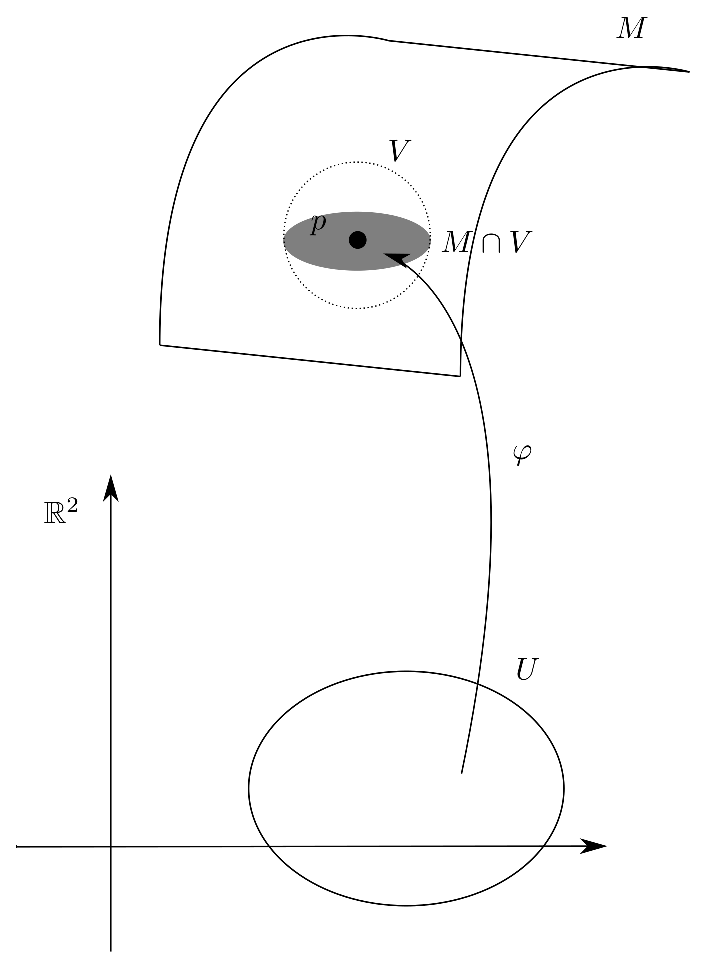
\includegraphics[scale=0.5]{graficos/parametrizacao.eps}
	\caption{Parametrização de uma superfície}
\end{figure}

\begin{obse}
	Quando $M \cap V = M$, $\varphi$ se chama de \emph{parametrização global}.
\end{obse}

\begin{exemplo}
Seja $f: U \subset \mathbb{R}^2 \rightarrow \mathbb{R}$ uma função diferenciável. Denote por $M$ seu gráfico
\begin{equation*}
    M = \text{Graf}(f) = \{ (x,f(x)): x \in U \}
\end{equation*}

Neste caso $M$ admite uma parametrização global. Defina $\varphi: U \rightarrow M$ pondo
\begin{equation*}
    \varphi(x) = (x,f(x)), x \in U
\end{equation*}
\end{exemplo}

\begin{defi}
Seja $\phi: V \subset \mathbb{R}^m \rightarrow \mathbb{R}^n$ uma aplicação diferenciável. Um ponto $p \in V$ é chamado de \emph{ponto crítico} de $\phi$ se $d\phi(p)$ \emph{não} é sobrejetora. Um ponto $q \in \mathbb{R}^n$ é chamado de \emph{valor crítico} de $\phi$ se existe algum ponto crítico de $\phi$ em $\phi^{-1}(q)$. Um ponto $q \in \mathbb{R}^n$ que não é valor crítico é chamado \emph{valor regular} para $\phi$.
\end{defi}

\begin{obse}
Quando $n=1$, um ponto $p \in V$ é ponto crítico de $\phi$ se e somente se $d\phi(p)=0$.
\end{obse}

\begin{teo}\label{preimagem_de_um_valor_regular}
Sejam $f: \mathbb{R}^3 \rightarrow \mathbb{R}$ uma função diferenciável e $c \in \mathbb{R}$ um valor regular para $f$. Então, o subconjunto
\begin{equation*}
    M = f^{-1}(c) \text{ é superfície regular.}
\end{equation*}
\end{teo}

\begin{proof}
Seja $p \in M$ tal que $p=(x_0,y_0,z_0)$, então $df(p) \neq 0$. Sem perdida de generalidade podemos dizer que $f_z(p) \neq 0$. Pelo Teorema da Função Implícita \cite[p.~296]{lima1985} \cite[p.~36]{montiel2009}, existem $U$ aberto de $\mathbb{R}^2$ tal que $(x_0,y_0) \in U$, $V$ aberto de $\mathbb{R}$ tal que $z_0 \in V$ e uma função diferenciável $g: U \rightarrow V$ tal que $g(x_0,y_0)=z_0$ e $f(x,y,g(x,y)) = c$ para todo $(x,y) \in U$.

Definamos $\varphi: U \rightarrow U \times V$ tal que $\varphi(x,y) = (x,y,g(x,y))$. Se ve que $\varphi$ é uma parametrização, portanto $M$ é uma superfície.
\end{proof}

\begin{exemplo}
Seja $f: \mathbb{R}^3 \rightarrow \mathbb{R}$ dada por $f(x) = \langle x,x \rangle$. Temos que $f$ é diferenciável e vale
\begin{equation*}
    df(p)v = 2 \langle p,v \rangle
\end{equation*}

para qualquer $p \in \mathbb{R}^3$ e para qualquer $v \in \mathbb{R}^3$. Disso decorre que $0 \in \mathbb{R}^3$ é o único ponto crítico de $f$. Note que
\begin{equation*}
    f(0) = 0 \neq 1.
\end{equation*}

Disso decorre, pelo teorema \ref{preimagem_de_um_valor_regular}, que a esfera $S^2 = f^{-1}(1)$ é uma superfície regular em $\mathbb{R}^3$.
\end{exemplo}

\begin{exemplo}
Seja $S^2 \subset \mathbb{R}^3$ a esfera unitária. Denote por $N$ seu polo norte, $N = (0,0,1)$ (ver figura \ref{projecao_estereografica}).

\begin{figure}

	\centering
	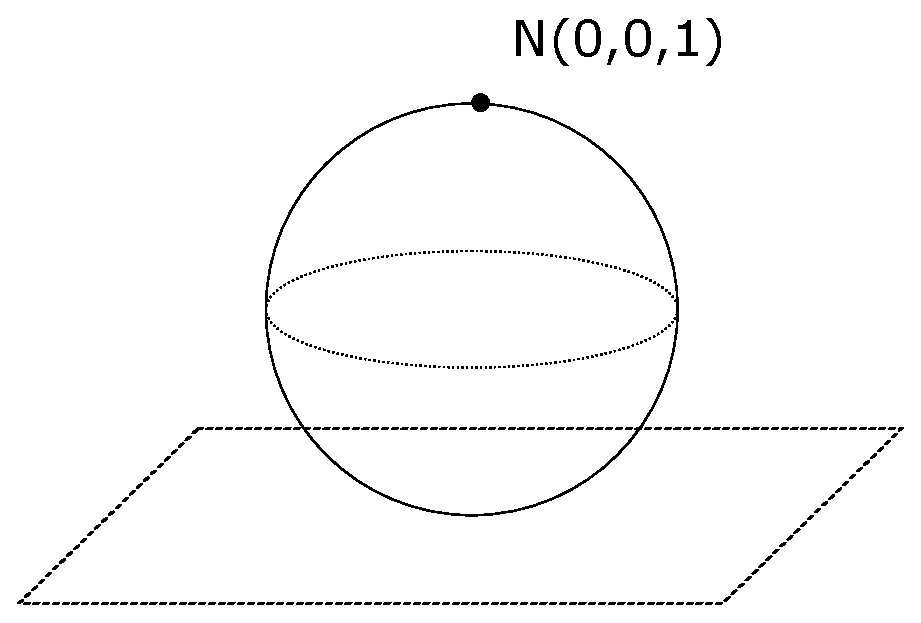
\includegraphics[scale=0.5]{graficos/projecao_estereografica.eps}
	\caption{Projeção estereográfica}
	\label{projecao_estereografica}
\end{figure}

Denote por $\pi_N$ a aplicação que associa a cada ponto $x \in S^2 \setminus \{N\}$ o ponto $\pi_N(x)$ no plano $x_3 = 0$, obtido pela interseção da semirreta que inicia no ponto $N$ e passa pelo ponto $x$ como o plano $x_3 = 0$. Os pontos da semirreta são da forma
\begin{equation*}
    N + t(x - N), t \geq 0.
\end{equation*}

Assim, a semirreta intercepta o plano $x_3 = 0$ quando
\begin{equation*}
    1 + t(x_3 - 1) = 0,
\end{equation*}

ou seja
\begin{equation*}
    t = \frac{1}{1 - x_3}
\end{equation*}

onde $x = (x_1, x_2, x_3)$. Por tanto
\begin{equation*}
    \pi_N(x) = \frac{1}{1-x_3} (x_1, x_2, 0)
\end{equation*}

Portanto $\pi_N$ é diferenciável. Por outro lado, a aplicação $\varphi: \mathbb{R}^2 \rightarrow S^2 \setminus \{N\}$ dada por
\begin{equation*}
	\varphi(x) = \left( \frac{2x_1}{\|x\|^2 + 1}, \frac{2x_2}{\|x\|^2 +1}, \frac{\|x\|^2 -1}{\|x\|^2 +1} \right)
\end{equation*} 

é diferenciável e vale $\pi_N \circ \varphi = \text{Id}$, ou seja, $\pi_N$ é um difeomorfismo.

Analogamente, podemos considerar $\pi_S$, onde $S=(0,0,-1)$.
\end{exemplo}

\begin{defi}
	Seja $M$ um conjunto. Uma \emph{carta local} em $M$ é uma bijeção $\varphi: U \rightarrow \varphi(U)$, onde $U$ é um subconjunto de $M$ e $\varphi(U)$ é um aberto de algum espaço euclideano $\mathbb{R}^n$.
\end{defi}

\begin{defi}
	Duas cartas locais em $M$, $(U, \varphi)$ e $(V, \psi)$, são \emph{compatíveis} se $U \cap V = \emptyset$ ou, se $U \cap V \neq \emptyset$, então $\varphi(U \cap V)$ e $\psi(U \cap V)$ sao abertos de $\mathbb{R}^n$ e a aplicação de transição $\psi \circ \varphi^{-1}$ é um difeomorfismo $C^{\infty}$.
\end{defi}

\begin{defi}
	Um \emph{atlas} $\mathcal{A}$ de dimensão $n$ em $M$ é um conjunto de cartas locais em $M$
	\begin{equation*}
		\mathcal{A} = \{ (U_{\alpha}, \varphi_{\alpha}):  \alpha \in I \}
	\end{equation*}
	
	onde cada $\varphi_{\alpha}(U_{\alpha})$ é aberto em $\mathbb{R}^n$ e $I$ é um conjunto de índices, duas a duas compatíveis e
	\begin{equation*}
		M = \bigcup_{\alpha \in I} U_{\alpha}
	\end{equation*}
\end{defi}

\begin{exemplo}
	Um atlas no espaco euclideano $\mathbb{R}^n$ é dado por
	\begin{equation*}
		\mathcal{A} = \{ (\mathbb{R}^n, \text{Id}) \}
	\end{equation*}
\end{exemplo}

\begin{exemplo}
	Na esfera $S^2$, um atlas é o conjunto
	\begin{equation*}
		\mathcal{A} = \{ (S^2 \setminus \{N\}, \pi_N), (S^2 \setminus \{S\}, \pi_S) \}
	\end{equation*}
	
	onde $\pi_N, \pi_S$ denotam as projeções estereográficas de $S^2$ relativas aos polos norte e sul respectivamente.
\end{exemplo}

\begin{defi}
	Uma carta local $\varphi$ em $M$ é dita \emph{compativel} com um atlas $\mathcal{A}$ em $M$ se $\varphi$ for compativel com todos os elementos do atlas $\mathcal{A}$.
\end{defi}

\begin{lema}
	Seja $\mathcal{A}$ um atlas em $M$. Se $(U, \varphi)$ e $(V, \psi)$ sao duas cartas locais em $M$, ambas compatíveis com $\mathcal{A}$, então ambas são compatíveis.
\end{lema}

\begin{proof}
	Se $U \cap V = \emptyset$, então as duas cartas são compatíveis. Supor que $U \cap V \neq \emptyset$, então existe $p \in U \cap V$. Como $\mathcal{A}$ é um atlas, então existe uma carta $(W, \rho) \in \mathcal{A}$ tal que $p \in W$. Pela hipótese, temos que $\varphi$ e $\psi$ são compatíveis com $\rho$, i.e., em $U \cap V \cap W$ temos que $\varphi \circ \rho^{-1}$ e $\rho \circ \psi^{-1}$ são difeomorfismos de classe $C^{\infty}$. Logo, $\varphi \circ \psi^{-1}$ é um difeomorfismo de classe $C^{\infty}$. Por tanto, $\varphi$ e $\psi$ são compatíveis. 
\end{proof}

\begin{defi}
	Um atlas $\mathcal{A}$ em $M$ é dito \emph{maximal} se nao está propriamente contido em nenhum atlas de $M$.
\end{defi}

\begin{lema}
	Dado um atlas $\mathcal{A}$ em $M$, existe um único atlas maximal $\mathcal{A}_{\text{max}}$ em $M$, com $\mathcal{A} \subset \mathcal{A_{\text{max}}}$.
\end{lema}

\begin{proof}
	Definamos $\mathcal{A}_{\text{max}}$ como o conjunto de todas as cartas compatíveis com $\mathcal{A}$. É claro que $\mathcal{A} \subset \mathcal{A_{\text{max}}}$. Para provar que $\mathcal{A_{\text{max}}}$ é um atlas peguemos $(U, \varphi)$ e $(V, \psi)$ duas cartas de $\mathcal{A_{\text{max}}}$. Pela definição de $\mathcal{A_{\text{max}}}$, temos que ambas cartas são compatíveis e portanto $\mathcal{A_{\text{max}}}$ é um atlas.
	
	Para provar que $\mathcal{A_{\text{max}}}$ é único vamos a pegar o atlas $\mathcal{B}$ tal que $\mathcal{A_{\text{max}}} \subset \mathcal{B}$. Como $\mathcal{A} \subset \mathcal{B}$, toda carta $(W, \rho) \in \mathcal{B}$ é compatível com $\mathcal{A}$, i.e., $\mathcal{B} \subset \mathcal{A_{\text{max}}}$. Portanto $\mathcal{A_{\text{max}}} = \mathcal{B}$.
\end{proof}

\begin{lema}
	Dado um atlas $\mathcal{A} = \{ (U_{\alpha}, \varphi_{\alpha}): \alpha \in I \}$ em $M$, existe uma única topologia $\tau_{\mathcal{A}}$ em $M$ que torna cada $U_{\alpha}$ aberto em $M$ e cada carta $\varphi_{\alpha}$ um homeomorfismo, i.e., $\tau_{\mathcal{A}}$ é a \emph{topologia induzida pelo atlas $\mathcal{A}$}.
\end{lema}

\begin{defi}
	Uma \emph{variedade suave} de dimensão $n$ é um par $(M, \mathcal{A})$, onde $M$ é um conjunto e $\mathcal{A}$ é um atlas maximal de dimensão $n$ em $M$ tal que a topologia induzida $\tau_{\mathcal{A}}$ seja de Hausdorff e satisfaça o segundo axioma da enumerabilidade.
\end{defi}

\begin{figure}
	\centering
	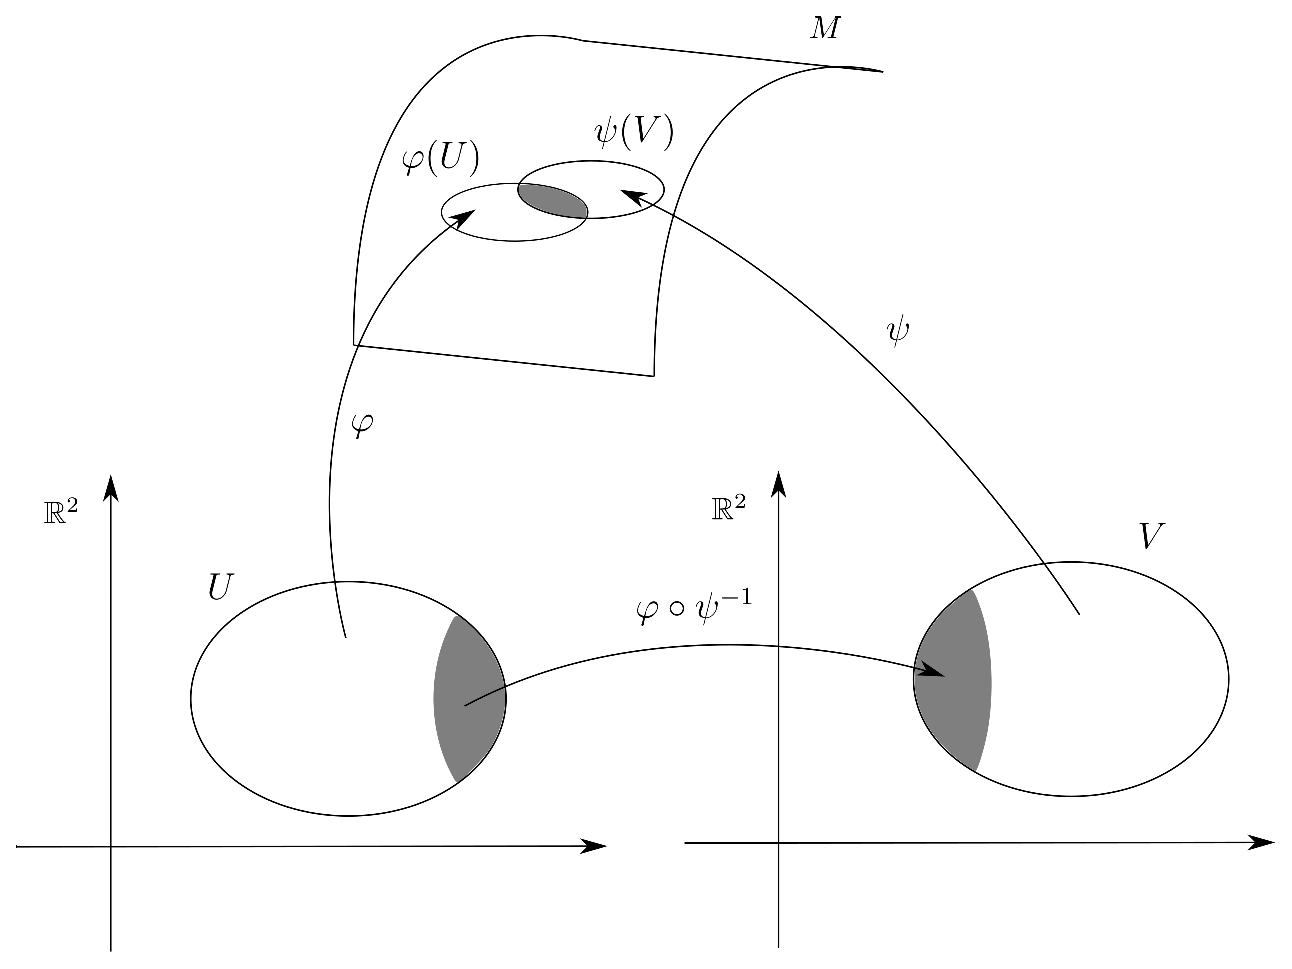
\includegraphics[scale=0.5]{graficos/cartas_compativeis.eps}
	\caption{Descrição gráfica de cartas compatíveis}
\end{figure}

Sejam $M$ uma superfície, $p \in M$ e $(U, \varphi)$ carta local em $M$ tal que $p \in U$. Como $\varphi(U)$ é aberto de $\mathbb{R}^2$, podemos expressar $\varphi$ como
\begin{equation*}
	\varphi(p) = (x(p), y(p)), \forall p \in U
\end{equation*}

As funções $x(p), y(p)$ são chamadas \emph{funções coordenadas} de $\varphi$ em $\mathbb{R}^2$.

\begin{nota}
	Para dizer que $\varphi$ está definido pelas funcoes coordenas $x$ e $y$ vamos escrever $\varphi \sim  (x,y)$.
\end{nota}

\begin{defi}
	O \emph{plano tangente} a $M$ num ponto $p \in M$ é o espaço vetorial real (abstrato) de dimensão 2 cuja base natural é
	\begin{equation*}
		\left\{ \frac{\partial}{\partial x} (p), \frac{\partial}{\partial y} (p) \right\}
	\end{equation*}
	
	onde $\frac{\partial}{\partial x}, \frac{\partial}{\partial y}$ são derivadas parciais de $\varphi$ em relação às coordenadas usuais de $\mathbb{R}^2$, i.e.
	\begin{align*}
		\frac{\partial}{\partial x} (p) = d \varphi^{-1} ( \varphi(p) ) e_1\\
		\frac{\partial}{\partial y} (p) = d \varphi^{-1} ( \varphi(p) ) e_2
	\end{align*}
	
	onde $\{ e_1,e_2 \}$ é a base canônica de $\mathbb{R}^2$. Além disso, identificando os vetores $\frac{\partial}{\partial x} (p), \frac{\partial}{\partial y} (p)$ como derivações temos
	\begin{align*}
		\frac{\partial}{\partial x} (p) (f) = \frac{\partial}{\partial x} \left( f \circ \varphi^{-1} \right) (\varphi(p))\\
		\frac{\partial}{\partial y} (p) (f) = \frac{\partial}{\partial y} \left( f \circ \varphi^{-1} \right) (\varphi(p))
	\end{align*}
	
	onde $f: M \rightarrow \mathbb{R}$ é uma função diferenciável.
\end{defi}

\begin{obse}
	Denote por $T_p M^*$ o espaço dual a $T_p M$, chamado o espaço cotangente a $M$ em $p$. O conjunto $T_p M^*$ também é um espaço vetorial cuja base é $\{ dx(p), dy(p)  \}$ dual à base $\{ \frac{\partial}{\partial x}(p), \frac{\partial}{\partial y}(p) \}$.
\end{obse}

\begin{lembrete}
	Se $E$ é um espaço vetorial real de dimensão $n$ com base $\{ e_1, e_2, \ldots, e_n \}$ sua base dual $\{ f_1, f_2, \ldots, f_n \} \subset E^*$ satisfaz
	\begin{equation*}
		f_i (e_j) = \delta_{ij}, 1 \leq i,j \leq n
	\end{equation*}
\end{lembrete}

	O conjunto
	\begin{equation*}
		TM = \bigcup_{p \in M} T_p M
	\end{equation*}
	
	dado pela união disjunta dos planos tangentes a $M$, é chamado de \emph{fibrado tangente} a $M$, admite uma estrutura de variedades suave de dimensão 4.

\section{Campos vetoriais}

\begin{defi}
	Seja $M^n$ uma variedade suave. Um \emph{campo vetorial} é uma aplicação diferenciável $X: M \rightarrow TM$ tal que $\pi \circ X = \text{Id}_M$.
	
	diagrama
	
	onde $\pi: TM \rightarrow M$ denota a projeção canônica
	\begin{equation*}
		\pi(p,v) = p
	\end{equation*}
\end{defi}

\begin{obse}
	A igualdade $\pi \circ X = \text{Id}_M$ significa que $X(p) \in T_p M$ para todo $p \in M$.
\end{obse}

\begin{nota}
	O conjunto dos campos vetoriais $X: M \rightarrow TM$ é denotado por $\mathfrak{X}(M)$.
\end{nota}

\begin{obse}
	Com as operações naturais
	\begin{align*}
		(X+Y)(p) &= X(p) + Y(p)\\
		(cX)(p) &= c X(p)
	\end{align*}
	
	onde $c \in \mathbb{R}$, o conjunto $\mathfrak{X}(M)$ torna-se um espaço vetorial real.
\end{obse}

\begin{obse}
	Dados $X \in \mathfrak{X}(M)$ e uma carta local $(U, \varphi$ em $M$, podemos escrever
	\begin{align*}
		X(p) = \sum_{i=1}^n a_i (p) \frac{\partial}{\partial x_i} (p), \forall p \in U
	\end{align*}
	
	onde $a_1, \ldots, a_n: U \rightarrow \mathbb{R}$ são funções e $\{ \frac{\partial}{\partial x_1}(p), \ldots, \frac{\partial}{\partial x_n}(p) \}$ é a base de $T_p M$ associada a $\varphi$, i.e.
	\begin{equation*}
		\frac{\partial}{\partial x_i} (p) = (d \varphi)^{-1}(\varphi(p)).e_i
	\end{equation*}
	
	onde $\{ e_1, \ldots, e_n \}$ é a base canônica de $\mathbb{R}^n$.
\end{obse}

Ver que $X \in \mathfrak{X}(M$ é diferenciável se e somente se os $a_1, \ldots, a_n$ são diferenciáveis em U.
	
\section{Formas diferenciáveis e orientação}

\begin{defi}
	Uma 1-forma $\omega$ em $M$ é uma aplicação diferenciável que a cada $p \in M$ associa um funcional linear $\omega(p): T_p M \rightarrow \mathbb{R}$.
\end{defi}

\begin{defi}
	Uma 2-forma $\omega$ em $M$ é uma aplicação diferenciável que associa a cada $p \in M$ uma 2-forma linear $\omega(p): T_p M \times T_p M \rightarrow \mathbb{R}$ alternada (antissimétrica)
	\begin{equation*}
		\omega(p) (v,w) = - \omega(p) (w,v) 
	\end{equation*}
\end{defi}

\begin{exemplo}
	Analisando $\mathbb{R}^2$ como variedade suave vemos que $T_p \mathbb{R}^2 \cong \mathbb{R}^2$. Além disso, o determinante
	\begin{align*}
		\text{det}: \mathbb{R}^2 \times \mathbb{R}^2 &\rightarrow \mathbb{R}\\
		(v,w) & \mapsto \det \left( \begin{matrix}
		v_1 & w_1\\
		v_2 & w_2
		\end{matrix} \right)
	\end{align*}
	
	é uma 2-forma.
\end{exemplo}

\begin{nota}
	\begin{align*}
		C^{\infty} &= \{ f: M \rightarrow \mathbb{R}: f \text{ é diferenciável} \}\\
		\mathfrak{X}(M) &= \{ X: M \rightarrow TM: X \text{ é um campo vetorial} \}\\
		\mathfrak{X}(M)^* &= \text{1-formas}
	\end{align*}
\end{nota}

\begin{defi}
	Seja $E$ um espaço vetorial com $v,w \in E$ e $f,g \in E^*$. O produto simétrico $\wedge$ está definido por
	\begin{align*}
		(f \wedge g) (v,w) &= f(v) g(w) - f(w) g(v)\\
		&= \text{Área}(v,w)
	\end{align*}
\end{defi}

\begin{defi}
	Uma superfície $M$ é dita \emph{orientável} se existe uma 2-forma $\omega$ em $M$ tal que $\omega(p) \neq 0$ para todo $p \in M$. Fixado uma tal 2-forma $\omega$, dizemos que o par $(M, \omega)$ é uma \emph{superfície orientada}.	
\end{defi}

A existência de uma 2-forma $\omega$ em $M$, com $\omega(p) \neq 0$ para todo $p \in M$, permite-nos decidir se a base $\{ \frac{\partial}{\partial x}(p), \frac{\partial}{\partial y}(p) \}$ do plano tangente $T_p M$, com $p \in U$, é positiva ou negativa (na orientação de $M$). Ou seja, se escrevemos
\begin{equation*}
	\omega(p) = h(p) dx(p) \wedge dy(p)
\end{equation*}

onde $h \in C^{\infty}(U)$, temos que $h$ tem sinal constante em $U$ porque $\omega$ não se anula. Logo, dizemos que:
\begin{itemize}
	\item $(U, \varphi)$ é \emph{orientada positiva} se $h >0$.
	\item $(U, \varphi)$ é \emph{orientada negativa} se $h<0$.
\end{itemize}

\begin{prop}
	Uma superfície $M$ é orientável se y somente se é possível escolher um atlas $\mathcal{A}$ em $M$ tal que o Jacobiano (o determinante da matriz jacobiana) de qualquer mudança de coordenadas é positiva.
\end{prop}

\begin{proof}
	contenidos...
\end{proof}	

\section{Variedades Riemannianas}

\begin{defi}
	Uma \emph{métrica Riemanniana} em uma variedade suave $M^n$ é uma correspondência $\langle , \rangle$ que associa a cada ponto $p \in M$, um produto interno $\langle , \rangle_p$ em $T_p M$ e que varia diferenciavelmente no sentido de que a função
	\begin{equation*}
		p \in M \mapsto \langle X(p), Y(p) \rangle_p
	\end{equation*}
	
	seja diferenciável para qualquer $X,Y \in \mathfrak{X}(M)$.
\end{defi}

\begin{defi}
	Uma \emph{variedade Riemanniana} é um par $(M, \langle , \rangle)$.
\end{defi}

\begin{obse}
	Dado uma carta local $(U, \varphi)$ em $M$ com $\varphi \sim (x_1, \ldots, x_n)$. Denote por
	\begin{equation*}
		dx_1, \ldots, dx_n
	\end{equation*}
	
	as 1-formas duais aos campos coordenados $\frac{\partial}{\partial x_1}, \ldots, \frac{\partial}{\partial x_n}$, ou seja,
	\begin{equation*}
		dx_i (p): T_p M \rightarrow \mathbb{R}
	\end{equation*}
	
	é o funcional linear dado por
	\begin{equation*}
		dx_i (p) \frac{\partial}{\partial x_j} = \delta_{ij}
	\end{equation*}
	
	onde $\delta_{ij} = 1$ quando $i=j$ e $\delta_{ij} = 0$ quando $i \neq j$. 
	
	Dados $p \in U$ e $v,w \in T_p M$, escrevamos
	\begin{align*}
		v &= \sum_{i=1}^n v_i \frac{\partial}{\partial x_i}(p) \text{ e }\\
		w &= \sum_{i=1}^n w_i \frac{\partial}{\partial x_i}(p)
	\end{align*}
	
	Usando a bilinearidade da métrica obtemos
	\begin{align*}
		\langle v,w \rangle_p &= \left\langle \sum_{i=1}^n v_i \frac{\partial}{\partial x_i}(p), \sum_{i=1}^n w_i \frac{\partial}{\partial x_i}(p) \right\rangle_p\\
		&= \sum_{i,j = 1}^n v_i w_j \left\langle \frac{\partial}{\partial x_i}(p), \frac{\partial}{\partial x_j}(p) \right\rangle_p\\
		&= \sum_{i,j=1}^n v_i w_j g_{ij}(p)
	\end{align*}
	
	onde $g_{ij}(p) = \left\langle \frac{\partial}{\partial x_i}(p), \frac{\partial}{\partial x_j}(p) \right\rangle_p$.
	
	Como $g_{ij} = g_{ji}$ e
	\begin{align*}
		dx_i (p) v &= dx_i (p) \left( \sum_{j=1}^n v_j \frac{\partial}{\partial x_j}(p) \right)\\
		&= v_i
	\end{align*}
	
	e
	\begin{equation*}
		dx_i (p) w = w_i
	\end{equation*}
	
	podemos escrever
	\begin{align*}
		\langle , \rangle &= \sum_{i,j=1}^n g_{ij} dx_i \otimes dx_j\\
		&= \sum_{i \leq j, i=1}^n \tilde{g}_{ij} dx_i dx_j
	\end{align*}
	
	onde $\tilde{g}_{ii} = g_{ii} $ e $\tilde{g}_{ij} = 2g_{ij}$ se $i \neq j$.
\end{obse}

\begin{exemplo}
	Em $\mathbb{R}^n$, identificamos
	\begin{equation*}
		\frac{\partial}{\partial x_i} (p) = e_i
	\end{equation*}
	
	com $1 \leq i \leq n$ para qualquer $p \in \mathbb{R}^n$. Assim, a métrica $\langle , \rangle$ em $\mathbb{R}^n$ é dada por
	\begin{align*}
		\left\langle \frac{\partial}{\partial x_i}(p), \frac{\partial}{\partial x_j}(p) \right\rangle_p &= \langle e_i, e_j \rangle_p\\
		&= \langle e_i, e_j \rangle\\
		&= \delta_{ij}
	\end{align*}
	
	ou seja
	\begin{align*}
		\langle , \rangle &= dx_1 dx_1 + \ldots + dx_n dx_n \\
		&= dx_1^2 + \ldots + dx_n^2
	\end{align*}
\end{exemplo}


\begin{exemplo}
	A métrica euclideana em $\mathbb{R}^2$ é dada por
	\begin{equation*}
		\langle , \rangle = dx^2 + dy^2
	\end{equation*}
	
	Passando para coordenadas polares
	\begin{align*}
		x &= r \cos \theta\\
		y &= r \sin \theta
	\end{align*}
	
	obtemos
	\begin{align*}
		dx &= \cos \theta dr - r \sin \theta d\theta\\
		dy &= \sin \theta dr + r \cos \theta d\theta
	\end{align*}
	
	Assim,
	\begin{align*}
		\langle , \rangle &= dx^2 + dy^2\\
		&= dr^2 + r^2 d\theta^2
	\end{align*}
\end{exemplo}

\begin{exemplo}
	Considere a superfície de rotação $M^2$ em $\mathbb{R}^3$ parametrizada por
	\begin{equation*}
		\varphi(s,\theta) = (a(s) \cos \theta, a(s) \sin \theta, b(s))
	\end{equation*}
	
	onde $a,b$ são funções diferenciáveis definidas em um intervalo aberto de $\mathbb{R}$, com $a>0$ e $\gamma(s) = (a(s),0,b(s))$ é a curva geratriz de $M^2$, com $\| \gamma'(s) \|^2 = (a'(s))^2 + (b'(s))^2 = 1$.
	
	Considere $M^2$ munida da métrica riemanniana $\langle , \rangle$ induzida de $\mathbb{R}^3$, i.e., cada plano tangente $T_p M$ está munido do produto interno usual de $\mathbb{R}^3$. Tais planos sao gerados pelas derivadas parciais
	\begin{align*}
		\frac{\partial \varphi}{\partial s} &= \varphi_s = (a'(s) \cos \theta, a'(s) \sin \theta, b'(s))\\
		\frac{\partial \varphi}{\partial \theta} &= \varphi_{\theta} = (-a(s) \sin \theta, a(s) \cos \theta, 0)
	\end{align*}
	
	Assim,
	\begin{align*}
		\langle , \rangle &= \langle \varphi_s, \varphi_s \rangle ds^2 + 2 \langle \varphi_s, \varphi_{\theta} \rangle ds d\theta + \langle \varphi_{\theta}, \varphi_{\theta} \rangle d\theta^2\\
		&= ds^2 + a(s)^2 d\theta^2
	\end{align*}
\end{exemplo}

\begin{exemplo}
	Seja $f: M \rightarrow N$ uma imersão, i.e., $f$ é uma aplicação diferenciável tal que
	\begin{equation*}
		df(p): T_p M \rightarrow T_{f(p)} N
	\end{equation*}
	
	é injetiva para qualquer $p \in M$. Suponha que $N$ esteja munida de uma métrica Riemanniana $\langle , \rangle^N$. Podemos definir uma métrica $\langle , \rangle^M$ em $M$
	\begin{equation*}
		\langle v,w \rangle_p^M := \langle df(p) v, df(p) w \rangle_{f(p)}^N
	\end{equation*}
	
	Neste caso, dizemos que $f$ é uma \emph{imersão isométrica}.
\end{exemplo}

\begin{teo}[Nash]
	Toda variedade suave $M$ pode ser mergulhada em algum espaço euclideano $\mathbb{R}^n$, i.e., existe uma imersão $f: M \rightarrow \mathbb{R}^n$ tal que sobre a imagem, $f$ é um homeomorfismo.
\end{teo}

\begin{corolario}
	Toda variedade suave $M$ pode ser munida de métrica Riemanniana.
\end{corolario}

\begin{proof}
	contenidos...
\end{proof}

\begin{defi}
	Uma \emph{conexão afim} em uma variedade suave $M$ é uma aplicação
	\begin{align*}
		\nabla: \mathfrak{X}(M) \times \mathfrak{X}(M) & \rightarrow \mathfrak{X}(M)\\
		(X,Y) & \mapsto \nabla_X Y
	\end{align*}
	
	que satisfaz:
	\begin{enumerate}
		\item $\nabla_X (Y+Z) = \nabla_X Y + \nabla_X Z$
		\item $\nabla_{fX+gY} Z = f \nabla_X Z + g \nabla_Y Z $
		\item $\nabla_X (fY) = f \nabla_X Y + X(f) Y$
	\end{enumerate}

para todo $X,Y,Z \in \mathfrak{X}(M)$ e $f,g \in C^{\infty}(M)$.
\end{defi}

\begin{lembrete}
	$X(f)(p) = df(p)X(p)$, i.e., $X: C^{\infty}(M) \rightarrow C^{\infty}(M)$.
\end{lembrete}

\begin{prop}\label{boa_definicao_conexao}
	Dados $p \in M$ e $X,Y \in \mathfrak{X}(M)$ o valor $(\nabla_X Y)(p)$ depende somente de $X(p)$ e da restrição de Y ao longo de uma curva diferenciável $\gamma: (-\epsilon, \epsilon) \rightarrow M$ com $\gamma(0)=p$ e $\gamma'(0)=X(p)$.
\end{prop}

\begin{figure}
	\centering
	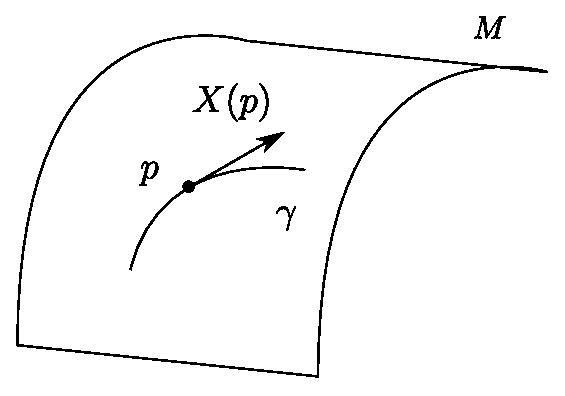
\includegraphics[scale=0.5]{graficos/curva_variedade.eps}
	\caption{Descrição da proposição \ref{boa_definicao_conexao}}
\end{figure}

\begin{proof}
	contenidos...
\end{proof}

\begin{nota}
	$\Gamma_{ij}^k =$ símbolos de Christoffel de $\nabla$ em relação a $(U,\varphi)$.
\end{nota}

\begin{obse}
	$(\nabla_X Y)(p) = \nabla_{X(p)} Y$
\end{obse}

\begin{teo}\label{levi-civita}
	Dado uma variedade Riemanniana $(M,\langle , \rangle)$, existe uma única conexão afim $\nabla$ em $M$ chamada de \emph{conexão de Levi-Civita} de $M$ que satisfaz:
	\begin{enumerate}
		\item $X \langle Y,Z \rangle = \langle \nabla_X Y,Z \rangle + \langle Y, \nabla_X Z\rangle$
		\item $\nabla_X Y - \nabla_Y X = [X,Y]$
	\end{enumerate}

onde $[X,Y]$ é o \emph{colchete de Lie} dado por
\begin{equation*}
	[X,Y] = X(Y(f)) - Y(X(f))
\end{equation*}
\end{teo}

\begin{proof}
	contenidos...
\end{proof}

\begin{obse}
	Dado um conexao $\nabla$ em $M$, satisfazendo a segunda propriedade do teorema \ref{levi-civita} e uma carta local $(U,\varphi)$ em $M$, com $\varphi \sim (x_1, \ldots, x_n)$, temos:
	\begin{equation*}
		\nabla_{\frac{\partial}{\partial x_i}} \frac{\partial}{\partial x_j} - \nabla_{\frac{\partial}{\partial x_j}} \frac{\partial}{\partial x_i} = \left[ \frac{\partial}{\partial x_i}, \frac{\partial}{\partial x_j} \right] =0
	\end{equation*}
	
	mostrando que $\Gamma_{ij}^k = \Gamma_{ji}^k$, para todo $1 \leq i,j \leq n$
\end{obse}

\begin{obse}
	Seja $(U,\varphi)$ uma carta local de $M$ tal que $\varphi \sim (x_1, \ldots,x_n)$. Então
	\begin{equation*}
		\left[\frac{\partial}{\partial x_i},\frac{\partial}{\partial x_j}\right](f) = \frac{\partial}{\partial x_i} \left(\frac{\partial f}{\partial x_j}\right) - \frac{\partial}{\partial x_j} \left(\frac{\partial f}{\partial x_i}\right)
	\end{equation*}
\end{obse}

\begin{obse}
	A conexão de Levi-Cevita de $\mathbb{R}^n$ coincide com a derivada usual de campos vetoriais em $\mathbb{R}^n$.
	
	De fato, sejam $(x_1,\ldots,x_n)$ as coordenadas usuais de $\mathbb{R}^n$. Temos
	\begin{align*}
		\left\langle \frac{\partial}{\partial x_i},\frac{\partial}{\partial x_j}\right\rangle &= \delta_{ij}\\
		\left[\frac{\partial}{\partial x_i},\frac{\partial}{\partial x_j}\right] &= 0
	\end{align*}
	
	Segue da formula de Koszul que
	\begin{equation*}
		\nabla_{\frac{\partial}{\partial x_i}} \frac{\partial}{\partial x_j} = 0, \forall 1 \leq i,j \leq n
	\end{equation*}
	
	implicando que $\Gamma_{ij}^k = 0, \forall i,j,k$. 
	
	Dados $X,Y \in \mathfrak{X}(\mathbb{R}^n)$, escrevamos
	\begin{align*}
		X &= \sum_{i=1}^n a_i \frac{\partial}{\partial x_i} \text{ e }\\
		Y &= \sum_{j=1}^n b_j \frac{\partial}{\partial x_j}
	\end{align*}
	
	onde $a_i,b_j \in C^{\infty}(\mathbb{R}^n)$. Usando a formula
	\begin{equation*}
		(\nabla_X Y)_{|U} = \sum_{k} \left(\sum_{i,j} a_i b_j \Gamma_{ij}^k + \sum_{i} a_i \frac{\partial b_k}{\partial x_i} \right) \frac{\partial}{\partial x_k}
	\end{equation*}
	
	obtemos
	\begin{align*}
		\nabla_X Y &= \sum_{k} \left(\sum_{i} a_i \frac{\partial b_k}{\partial x_i} \right) \frac{\partial}{\partial x_k}\\
		&= \sum_{k} X(b_k) \frac{\partial}{\partial x_k}\\
		&= X(Y)
	\end{align*}
\end{obse}

\begin{exemplo}
	Seja $\mathbb{R}_+^2 = \{(x,y) \in \mathbb{R}^2: y>0\}$ e $\langle,\rangle = \frac{1}{y^2} \left(dx^2+dy^2\right)$. Vamos calcular $\nabla_{\frac{\partial}{\partial x_1}} \frac{\partial}{\partial x_1}$, $\nabla_{\frac{\partial}{\partial x_2}} \frac{\partial}{\partial x_2}$ e $\nabla_{\frac{\partial}{\partial x_1}} \frac{\partial}{\partial x_2}$
\end{exemplo}

\section{Superfícies de Rienmann}

\begin{defi}
	Uma superfície Riemanniana é um par $(M, \langle, \rangle)$, onde $M$ é uma variedade suave de dimensão 2 e $\langle, \rangle$ é uma métrica Riemanniana em $M$.
\end{defi}

Isso significa que $\langle,\rangle$ é um $(2,0)-$tensor simétrico e positivo definido. Ou seja, para qualquer $p \in M$, $\langle,\rangle_p: T_pM \times T_pM \rightarrow \mathbb{R}$ é um produto interno positivo definido em $T_pM$.

Dada uma carta local $(U,\varphi)$ em $M$, para cada $p \in M$, podemos expressar a métrica $\langle,\rangle$ como:
\begin{align*}
	\langle,\rangle_p &= E dx \otimes dx + F (dx \otimes dy + dy \otimes dx) + G dy \otimes dy
\end{align*}

onde $E,F,G \in C^{\infty}(U)$. De forma simplificada
\begin{equation*}
	\langle,\rangle = E dx^2 + 2F dx dy + G dy^2
\end{equation*}

Lembre que, dado uma superfície Riemanniana $(M,\langle,\rangle)$, existe uma única conexão afim $\nabla$ em $M$, a conexão de Levi-Civita de $M$, que satisfaz:
\begin{enumerate}
	\item $\nabla$ é compatível com $\langle,\rangle$:
	\begin{equation}\label{conexao_prop_derivada}
		X \langle Y,Z \rangle = \langle \nabla_X Y, Z \rangle + \langle Y, \nabla_X Z \rangle
	\end{equation}
	
	\item $\nabla$ é simétrica:
	\begin{equation*}
		\nabla_X Y - \nabla_Y X = [X,Y]
	\end{equation*}
	
	onde $[,]$ é o \emph{colchete de Lie} em $\mathfrak{X}(M)$.
\end{enumerate}

Dada uma carta local $(U,\varphi)$ em $M$, com $\varphi \cong (x,y)$, temos os campos coordenados $\frac{\partial}{\partial x}, \frac{\partial}{\partial y}$ dados por
\begin{align*}
	\frac{\partial}{\partial x}(p) &= d \varphi^{-1}(p) e_1\\
	\frac{\partial}{\partial y}(p) &= d \varphi^{-1}(p) e_2
\end{align*}

onde $\{e_1,e_2\}$ é a base canônica de $\mathbb{R}^2$.

Considere os símbolos de Christoffel $\Gamma_{ij}^k \in C^{\infty}(U)$ da conexão Levi-Civita $\nabla$ de $M$, associada a $\langle.\rangle$, dados por
\begin{equation}
	\begin{split}
		\nabla_{\frac{\partial}{\partial x}} \frac{\partial}{\partial x} &= \Gamma_{11}^1 \frac{\partial}{\partial x} + \Gamma_{11}^2 \frac{\partial}{\partial y}\\\label{christoffel}
		\nabla_{\frac{\partial}{\partial x}} \frac{\partial}{\partial y} &= \Gamma_{12}^1 \frac{\partial}{\partial x} + \Gamma_{11}^2 \frac{\partial}{\partial y}\\
		\nabla_{\frac{\partial}{\partial y}} \frac{\partial}{\partial y} &= \Gamma_{22}^1 \frac{\partial}{\partial x} + \Gamma_{2}^2 \frac{\partial}{\partial y}
	\end{split}	
\end{equation}

\begin{prop}
	Os símbolos de Christoffel são dados por:
	\begin{align*}
		\Gamma_{11}^1 &= \frac{1}{2(EG-F^2)} (GE_x - 2FF_x + FE_y)\\
		\Gamma_{11}^2 &= -\frac{1}{2(EG-F^2)} (EE_y - 2EF_x + FE_x)\\
		\Gamma_{12}^1 &= \frac{1}{2(EG-F^2)} (GE_y - FG_x)\\
		\Gamma_{12}^2 &= \frac{1}{2(EG-F^2)} (EG_x - FE_y)\\
		\Gamma_{22}^1 &= \frac{1}{2(EG-F^2)} (GG_x - 2GF_y + FG_y)\\
		\Gamma_{22}^2 &= \frac{1}{2(EG-F^2)} (EG_y - 2FF_y + FG_x)
	\end{align*}
\end{prop}

\begin{proof}
	Usando \eqref{christoffel}, temos
	\begin{align*}
		\left\langle \nabla_{\frac{\partial}{\partial x}} \frac{\partial}{\partial y}, \frac{\partial}{\partial x} \right\rangle &= \Gamma_{12}^1 E + \Gamma_{12}^2 F\\
		\left\langle \nabla_{\frac{\partial}{\partial x}} \frac{\partial}{\partial y}, \frac{\partial}{\partial y} \right\rangle &= \Gamma_{12}^1 F + \Gamma_{12}^2 G
	\end{align*}
	
	Por outro lado, como $\left[ \frac{\partial}{\partial x}, \frac{\partial}{\partial y} \right] = 0$, e usando \eqref{conexao_prop_derivada}, temos
	\begin{align*}
		\left\langle \nabla_{\frac{\partial}{\partial x}} \frac{\partial}{\partial y}, \frac{\partial}{\partial x} \right\rangle &= \left\langle \nabla_{\frac{\partial}{\partial y}} \frac{\partial}{\partial x}, \frac{\partial}{\partial x} \right\rangle\\
		&= \frac{1}{2}	\pdiff{y} \innerproduct{\pdiff{x}}{\pdiff{x}}\\
		&= \frac{1}{2} E_y\\
		\innerproduct{\conection{\pdiff{x}}{\pdiff{y}}}{\pdiff{y}} &= \frac{1}{2} \pdiff{x} \innerproduct{\pdiff{y}}{\pdiff{y}}\\
		&= \frac{1}{2} G_x
	\end{align*}
	
	Temos assim o seguinte sistema
	\begin{align*}
		\christoffel{12}{1} E + \christoffel{12}{2} F &= \frac{1}{2} E_y\\
		\christoffel{12}{1} F + \christoffel{12}{2} G &= \frac{1}{2} G_x
	\end{align*}
	
	ou seja,
	\begin{equation*}
		\left( \begin{matrix}
		E & F\\
		F & G
		\end{matrix} \right) \left( \begin{matrix}
		\christoffel{12}{1}\\
		\christoffel{22}{2}
		\end{matrix} \right) = \frac{1}{2} \left( \begin{matrix}
		E_y\\
		G_x
		\end{matrix} \right)
	\end{equation*}
	
	Resolvendo tal sistema $(EG-F^2 > 0)$, obtemos expressões para $\christoffel{12}{1}$ e $\christoffel{12}{2}$.
\end{proof}

\begin{defi}
	O \emph{tensor de curvatura} de uma superfície Riemanniana $M$ é a aplicação
	\begin{equation*}
		\mathcal{R}: \vectorfields{M} \times \vectorfields{M} \times \vectorfields{M} \rightarrow \vectorfields{M}
	\end{equation*}
	
	dada por
	\begin{equation*}
		\mathcal{R}(X,Y) Z = \conection{X}{\conection{Y}{Z}} - \conection{Y}{\conection{X}{Z}} - \conection{\liebrackets{X}{Y}}{Z}
	\end{equation*}
	
	para qualquer $X,Y,Z \in \vectorfields{M}$.
\end{defi}

\begin{prop}
	Valem as seguintes propriedades:
	\begin{enumerate}[i)]
		\item $\mathcal{R}$ é um tensor, i.e., $\mathcal{R} \in \smoothfunction{M}$ e é linear em $X,Y,Z$.
		\item $\mathcal{R}$ é antissimétrico em $X,Y$, i,e., $\mathcal{R}(X,Y) = -\mathcal{R}(Y,X)$.
		\item $\innerproduct{\mathcal{R}(X,Y),Z}{W} = -\innerproduct{\curvaturetensor{Z}{W}{X}}{Y}$.
		\item $\curvaturetensor{X}{Y}{Z} + \curvaturetensor{Y}{Z}{X} + \curvaturetensor{Z}{X}{Y} = 0$ (Primeira identidade de Bianchi).
	\end{enumerate}
\end{prop}

\begin{defi}
	Seja $(M,\innerproduct{}{})$ uma superficial Riemanniana com tensor de curvatura $\mathcal{R}$.
	
	A \emph{curvatura Gaussiana} (ou curvatura intrínseca) $K$ de $M$, associada a $\innerproduct{}{}$ é definida por:
	\begin{equation*}
		K(p) = \frac{\innerproduct{\curvaturetensor{X}{Y}{Y}}{X}}{\norm{X \wedge Y}^2}
	\end{equation*}
	
	onde $p \in M$, $X,Y \in T_pM$ são vetores linearmente independentes e
	\begin{equation*}
		\norm{X \wedge Y}= \sqrt{\norm{X}^2 \norm{Y}^2 - \innerproduct{X}{Y}^2}
	\end{equation*}
\end{defi}

\begin{prop}
	O valor de $K(p)$ não depende da escolha de $X,Y$.
\end{prop}

\begin{proof}
	contenidos...
\end{proof}


\begin{obse}
	O tensor de curvatura $\mathcal{R}$ é completamente determinado por $K$, pois
	\begin{align*}
		\curvaturetensor{X}{Y}{Z} &= K(X \wedge Y) Z\\
		&= K(\innerproduct{Y}{Z} X - \innerproduct{X}{Z} Y)
	\end{align*}
	
	para qualquer $X,Y,Z \in \vectorfields{M}$.
\end{obse}

\begin{obse}
	Dado uma carta local $(U,\varphi)$ em $M$, com $\varphi \cong (x,y)$, existe uma relação entre os símbolos de Christoffel e o tensor de curvatura $\mathcal{R}$ associado a $\varphi$.
	
	Como $\liebrackets{\pdiff{x}}{\pdiff{y}} = 0$, e usando \eqref{christoffel}. temos:
	\begin{equation*}
%		\begin{split}
			\curvaturetensor{\pdiff{x}}{\pdiff{y}}{\pdiff{y}} = \conection{\pdiff{x}}{\conection{\pdiff{y}}{\pdiff{y}}} - \conection{\pdiff{y}}{\conection{\pdiff{x}}{\pdiff{y}}}\\
%			=& \conection{\pdiff{x}}{\christoffel{22}{1} \pdiff{x} + \christoffel{22}{2} \pdiff{y}} - \conection{\pdiff{y}}{\christoffel{12}{1} \pdiff{x} + \christoffel{12}{2} \pdiff{y}}\\
%			=& \left( \partialdiff{\christoffel{12}{1}}{x} - \partialdiff{\christoffel{12}{1}}{y} \right) \pdiff{x} + \left( \partialdiff{\christoffel{22}{2}}{x} - \partialdiff{\christoffel{12}{2}}{y} \right) \pdiff{y}\\
%			& + \christoffel{22}{1} \conection{\pdiff{x}}{\pdiff{x}} + \christoffel{22}{2} \conection{\pdiff{x}}{\pdiff{y}}\\
%			& - \christoffel{12}{1} \conection{\pdiff{y}}{\pdiff{x}} - \christoffel{12}{2} \conection{\pdiff{y}}{\pdiff{y}}
%		\end{split}	
	\end{equation*}
	
	Usando \eqref{christoffel} temos que:
	\begin{multline*}
		%\begin{split}
			\curvaturetensor{\pdiff{x}}{\pdiff{y}}{\pdiff{y}} =\\
			 \left( \partialdiff{\christoffel{12}{1}}{x} - \partialdiff{\christoffel{12}{1}}{y} +\christoffel{22}{1} \christoffel{11}{1} + \christoffel{22}{2} \christoffel{12}{2} - \christoffel{12}{1} \christoffel{12}{1} - \christoffel{12}{2} \christoffel{22}{1} \right) \pdiff{x} \\
			 + \left( \partialdiff{\christoffel{22}{2}}{x} - \partialdiff{\christoffel{12}{2}}{y} + \christoffel{22}{1} \christoffel{11}{2} - \christoffel{12}{1} \christoffel{12}{1} \right) \pdiff{y}
		%\end{split}	
	\end{multline*}
	
	Agora tomando o produto interno com $\pdiff{x}$:
	\begin{multline*}
		K =\\
		\frac{E}{EG-F^2} \left( \partialdiff{\christoffel{12}{1}}{x} - \partialdiff{\christoffel{12}{1}}{y} +\christoffel{22}{1} \christoffel{11}{1} + \christoffel{22}{2} \christoffel{12}{2} - \christoffel{12}{1} \christoffel{12}{1} - \christoffel{12}{2} \christoffel{22}{1} \right) \\
		+ \frac{F}{EG-F^2} \left( \partialdiff{\christoffel{22}{2}}{x} - \partialdiff{\christoffel{12}{2}}{y} + \christoffel{22}{1} \christoffel{11}{2} - \christoffel{12}{1} \christoffel{12}{1} \right)
	\end{multline*}
\end{obse}

\begin{obse}
	O plano $\realnumbers^2$ pode ser identificado com $\complexnumbers$ através do isomorfismo
	\begin{equation*}
		(x,y) \in \realnumbers^2 \mapsto x + iy \in \complexnumbers
	\end{equation*}
	
	Uma função $f: U \rightarrow \complexnumbers$, definida num aberto $U \subset \complexnumbers$, é dita $\complexnumbers-$diferenciável em $z_0 \in U$ se existe o limite
	\begin{equation*}
		f'(z_0) = \lim_{z \rightarrow z_0} \frac{f(z) - f(z_0)}{z - z_0}
	\end{equation*}
	
	Se $f$ é $\complexnumbers-$diferenciável em todo $z \in U$ dizemos que $f$ é holomorfa.
\end{obse}

\begin{defi}
	Uma superfície conexa $M$ é chamada \emph{superfície de Riemann} se existe um atlas de cartas locais $\mathcal{A} = \{ (U_i,\varphi_i): i \in I \}$ de $M$ tal que $\varphi_i(U_i) \subset \complexnumbers$ e $\varphi_j \circ \varphi_i^{-1}$ é holomorfa, quando $U_i \cap U_j \neq \emptyset$.
\end{defi}

\begin{teo}[Existência de parâmetros isotermos]
	Considere uma superfície de Riemann $(M, \innerproduct{}{})$. Então, para qualquer $p \in M$, existe uma carta local $(U,\varphi)$ em $M$, com $p \in U$ e $\varphi \sim (x,y)$, e uma função diferenciável $\rho: U \rightarrow \realnumbers$ tais que:
	\begin{gather*}
		\innerproduct{\pdiff{x}}{\pdiff{x}} = \innerproduct{\pdiff{y}}{\pdiff{y}} = e^{\rho(x,y)}\\
		\innerproduct{\pdiff{x}}{\pdiff{y}} = 0
	\end{gather*}
\end{teo}

\begin{teo}
	Seja $M$ uma superfície Riemanniana orientada e considere um atlas $\mathcal{A} = \{ (U_p,\varphi_p): p \in M \}$ de modo que cada carta $(U_p,\varphi_p)$ é isoterma e orientada positiva. Então, as mudanças de coordenadas são holomorfas, logo $M$ é uma superfície de Riemann.
\end{teo}

\begin{prop}
	Seja $f: M \rightarrow \complexnumbers$ uma função diferenciável. Então $f$ é holomorfa se e somente se $\partialdifffrac{f}{z} = 0$ para toda carta local $(U,\varphi)$ em $M$.
\end{prop}